\documentclass[11pt]{article}
\usepackage[margin=1in]{geometry}
\usepackage{mathptmx}
\usepackage{url}
\Urlmuskip=0mu plus 1mu
\usepackage{titlesec}
\usepackage{setspace}
\usepackage{parskip}
\usepackage{microtype}
\usepackage{enumitem}
\usepackage{tikz}
\usepackage{caption}
\usepackage{graphicx}
\usepackage{amssymb}
\usetikzlibrary{arrows.meta, positioning, fit, backgrounds, shapes.geometric, calc}

\captionsetup{labelfont=bf, font=small}

\titleformat{\section}{\normalfont\bfseries\large}{\thesection}{1em}{}
\titlespacing*{\section}{0pt}{12pt}{6pt}
\titleformat{\subsection}{\normalfont\bfseries}{\thesubsection}{1em}{}
\titlespacing*{\subsection}{0pt}{10pt}{4pt}

\begin{document}
\pagestyle{empty}

\begin{center}
{\LARGE\bfseries Constraint Optimization through RTL Enhancement Using Generative AI}\\[8pt]
{\large\bfseries Team Timing Blinders}\\[6pt]
{\large Nagarjun BV \quad (25M1157)}\\[2pt]
{\large Shubhanshu Shivhare \quad (25M1173)}\\[4pt]
{\normalsize M.Tech, Electronic Systems, IIT Bombay --- 2nd Year}\\[4pt]
{\small Astera Labs Nebula 2026, Digital Track}
\end{center}

\vspace{8pt}

\section*{Motivation}

Closing timing on a block is the same manual loop, every time: read the STA
report, find the path that missed, pick a fix, edit the RTL by hand,
re-synthesize, check if it helped. Repeat.

\begin{itemize}[leftmargin=1.4em, itemsep=2pt]
\item \textbf{The fix is always one of four techniques:} pipelining, register
retiming, logic restructuring, or FSM re-encoding.
\item \textbf{This can be automated.} It is still done by hand today only
because nobody trusts a tool to rewrite RTL safely without a human
double-checking it.
\item \textbf{We remove that trust problem.} Every automated edit is checked
and mathematically proven to preserve the design's original behavior before
it is accepted --- so the system is safe to run without a human reviewing
each edit.
\end{itemize}

These four are not the only timing fixes that exist --- they are the only
ones GenAI is asked to propose. Gate-level fixes (cell sizing, buffer
insertion, and similar) are already handled automatically by the synthesis
and place-and-route tools themselves; GenAI is scoped to the RTL-level
structural edits those tools cannot make on their own.

\begin{center}
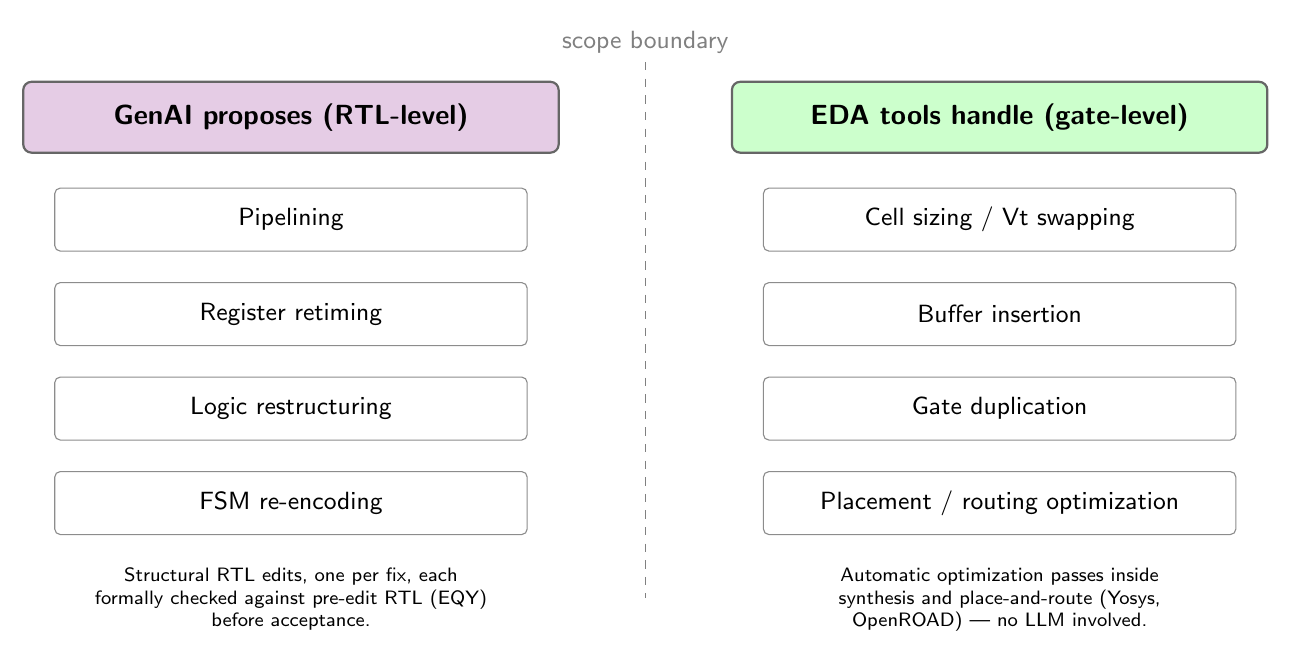
\includegraphics[width=0.95\linewidth]{technique_spectrum.png}
\captionof{figure}{Scope split: GenAI proposes RTL-level structural edits; EDA tools (Yosys/OpenROAD) continue to handle gate-level optimization automatically, as they already do today.}
\end{center}

\section*{Closed-Loop Architecture}

One loop, five gates, each one checked before the design is allowed to touch
the next stage.

\begin{itemize}[leftmargin=1.4em, itemsep=3pt]
\item \textbf{A lint gate} runs first, on every RTL candidate, before it is
allowed anywhere near synthesis: Verilator/slang catch structural issues
(unused signals, width mismatches, latch inference). Rule-matched issues get
a deterministic, zero-token auto-fix; unmatched ones fall through to a small
GenAI lint-repair pass. Either way, nothing reaches synthesis until lint
passes.
\item \textbf{\texttt{run\_sta}} wraps OpenSTA, turns a raw timing report into
ranked critical paths with slack --- in a form an LLM can actually read.
\item \textbf{\texttt{propose\_and\_apply\_edit}} hands that path, and only
that path's RTL, to the model, constrained to emit exactly one of the four
techniques above as edited Verilog --- never prose, never a suggestion the
model then has to also implement correctly by hand. Every such edit is itself
checked with EQY/SymbiYosys against the pre-edit RTL before it is accepted;
fail that check and the edit is discarded, no exceptions.
\item \textbf{\texttt{resynth\_and\_check}} re-synthesizes an accepted edit in
Yosys and re-runs OpenSTA to confirm timing/area/power actually improved.
This is a second, separate equivalence gate from the one above: it checks the
\emph{synthesized netlist} against the RTL that produced it --- proving the
synthesis step itself was behavior-preserving, not just the LLM's edit --- and
only a pass here is allowed to proceed to floorplanning.
\item \textbf{A second, advisory GenAI pass} runs downstream of
place-and-route (placement, CTS, routing, STA) and surfaces physical-design
suggestions from the accumulated PPA trail. It observes but does not silently
rewrite RTL --- the two formally-gated checks above stay the only path that
mutates the design.
\end{itemize}

Papers in this space (ViTAD~\cite{vitad}, SymRTLO~\cite{symrtlo},
TimingLLM~\cite{timingllm}) get as far as diagnosing a violation and
proposing a fix; none of them formally prove the fix didn't break the design
before calling it a result. That gap is where this project sits.

\begin{center}
\small
\begin{tabular}{lcccc}
\hline
\textbf{System} & \textbf{Diagnoses} & \textbf{Proposes} & \textbf{Formal} & \textbf{PPA} \\
 & \textbf{violation} & \textbf{RTL fix} & \textbf{equiv. gate} & \textbf{before/after} \\
\hline
ViTAD~\cite{vitad} (2025)      & \checkmark & \checkmark & $\times$   & $\times$ \\
SymRTLO~\cite{symrtlo} (2025)     & \checkmark & \checkmark & $\times$   & $\times$ \\
TimingLLM~\cite{timingllm}         & \checkmark & $\times$   & $\times$   & $\times$ \\
\textbf{Nebula (this work)} & \checkmark & \checkmark & \checkmark & \checkmark \\
\hline
\end{tabular}
\captionof{table}{No cited system formally proves an LLM-proposed RTL edit is behavior-preserving before reporting a result --- the EQY/SymbiYosys gate is what this project adds.}
\end{center}

\begin{center}
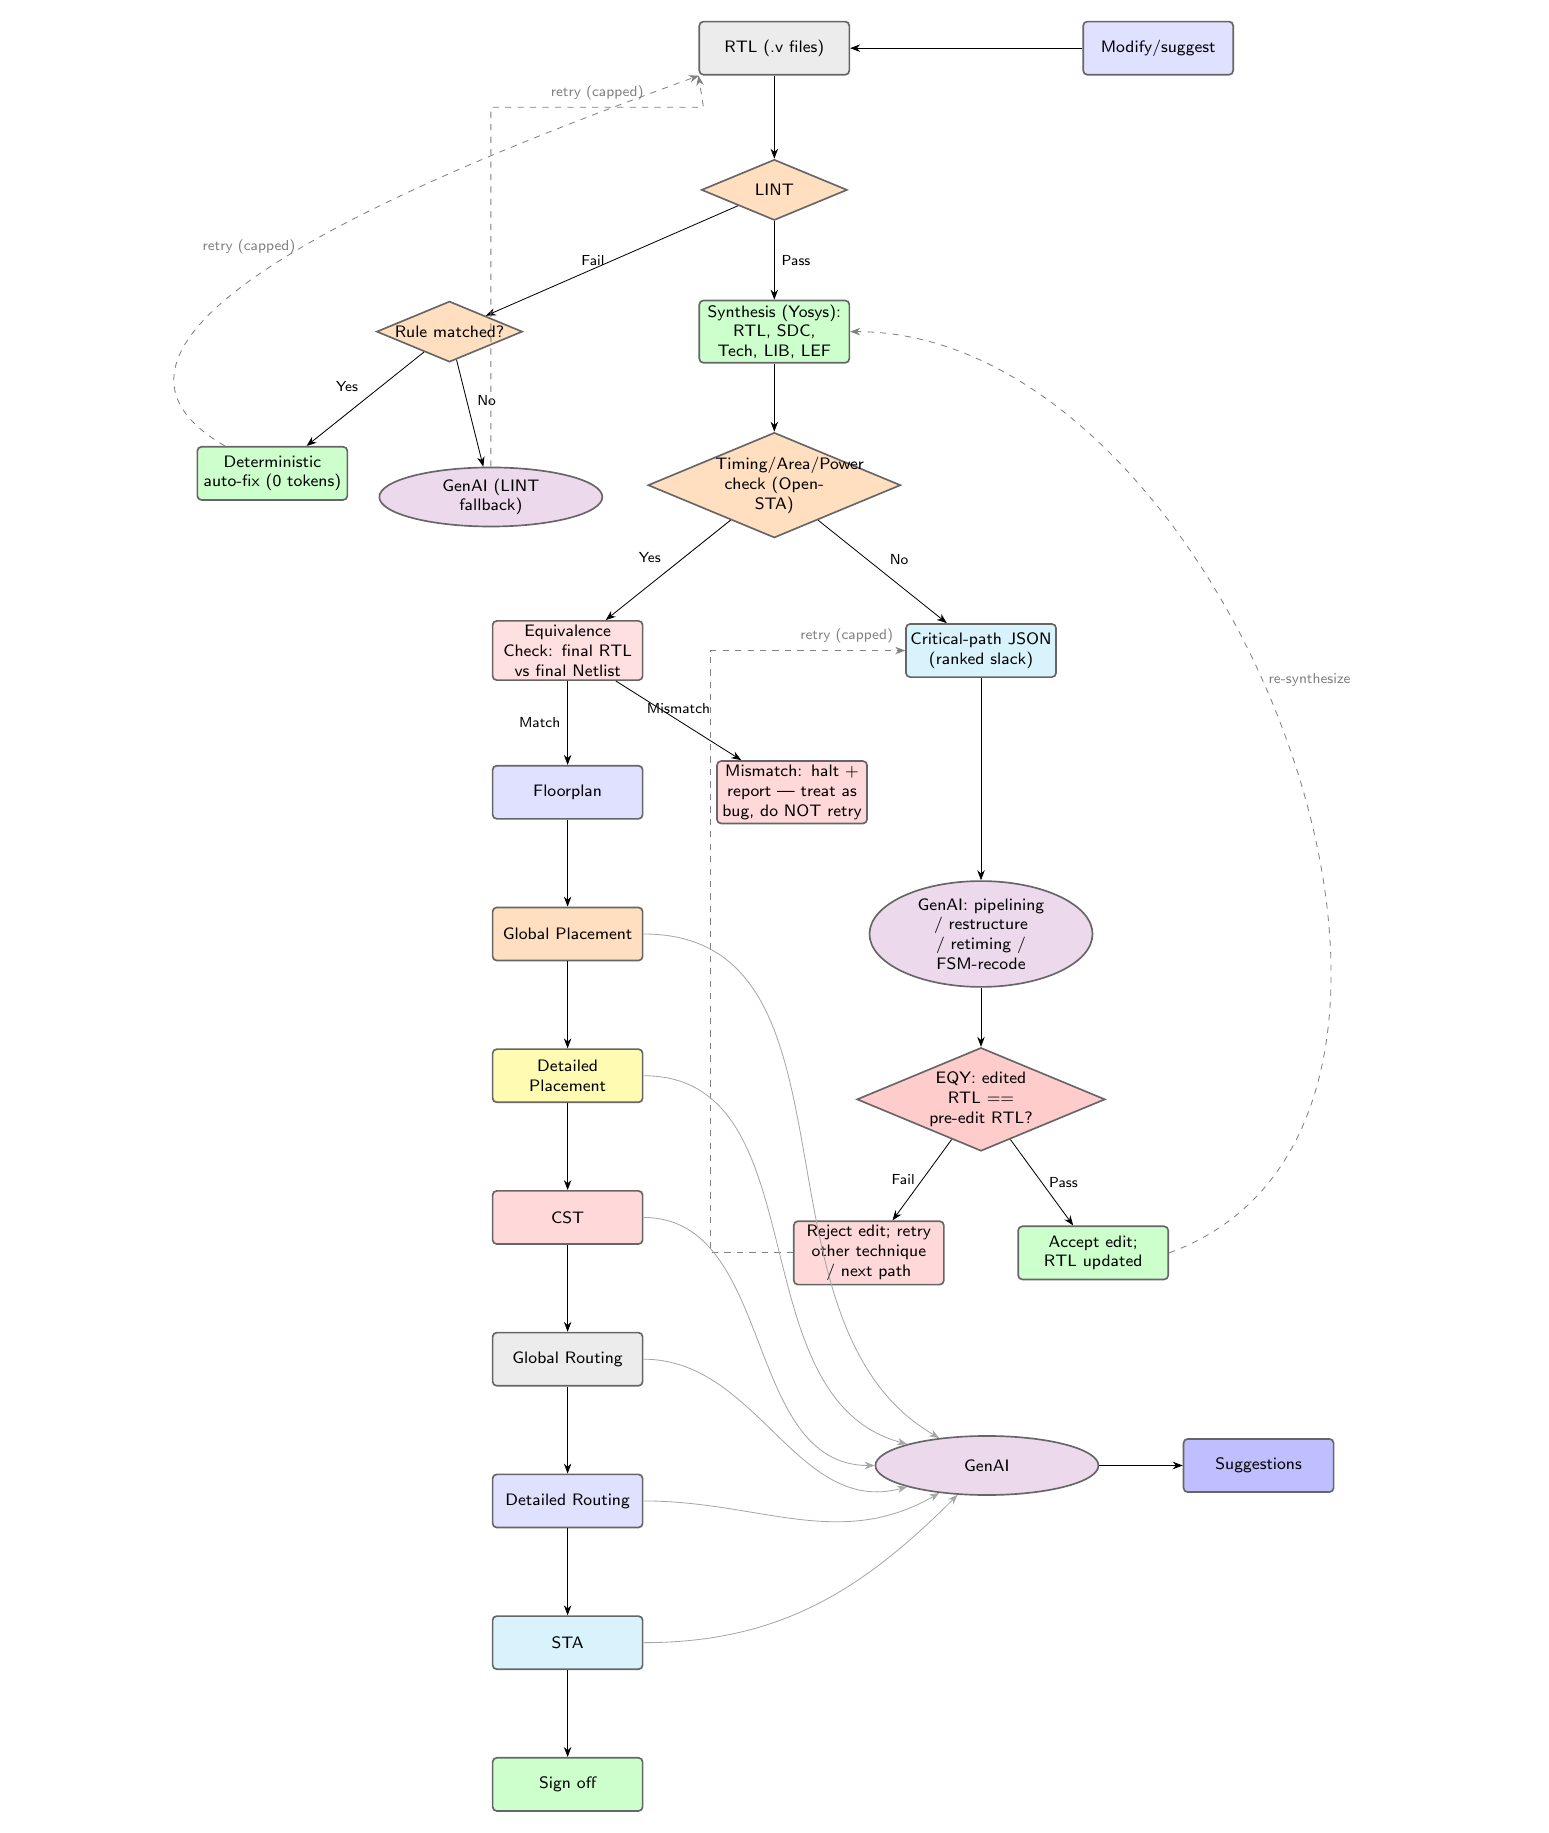
\includegraphics[width=0.78\linewidth]{flowchart_corrected.png}
\captionof{figure}{Closed-loop RTL-fix pipeline. Every GenAI edit is checked against pre-edit RTL before acceptance; the final equivalence check gates entry to floorplanning, and a mismatch there halts and reports rather than retrying.}
\end{center}

\section*{Benchmark Design}

The benchmark (Figure~2) is a small SoC sized to make the loop earn its
numbers, not a toy that happens to synthesize cleanly: five independent
asynchronous master clock domains, generated clocks at multiple divide
ratios per domain (Figure~3), clock-domain crossings between every
peripheral and the core, roughly 50{,}000 standard cells post-synthesis.

A RISC-V core with split L1 instruction/data caches and a DMA engine sits on
domain 1 (\texttt{Clk\_1}), talking to the rest of the system through a
shared AXI interconnect and driving generated clocks at three ratios
(1.25, 1.5, 2) --- the fractional ratios in particular push the divider logic
past a simple counter into pulse-swallow-style generation, deliberately
raising the bar on what ``clock divider logic'' has to mean here. Four
peripherals hang off the interconnect, each in its own asynchronous domain,
crossing through dedicated FIFOs rather than direct AXI taps: an FP4
dot-product accelerator on domain 2 (divide-by-2), a GPIO block on domain 3
spanning seven ratios (2, 4, 8, 16, 32, 64, 128 --- seven octave steps), a
timer on domain 4 (2, 4, 8), and a UART on domain 5 (2, 4, 6). Every one of those five
domain boundaries is a real CDC crossing the loop has to reason about
correctly when it proposes a retiming or pipelining edit near a domain edge
--- not a simulated one.

\begin{center}
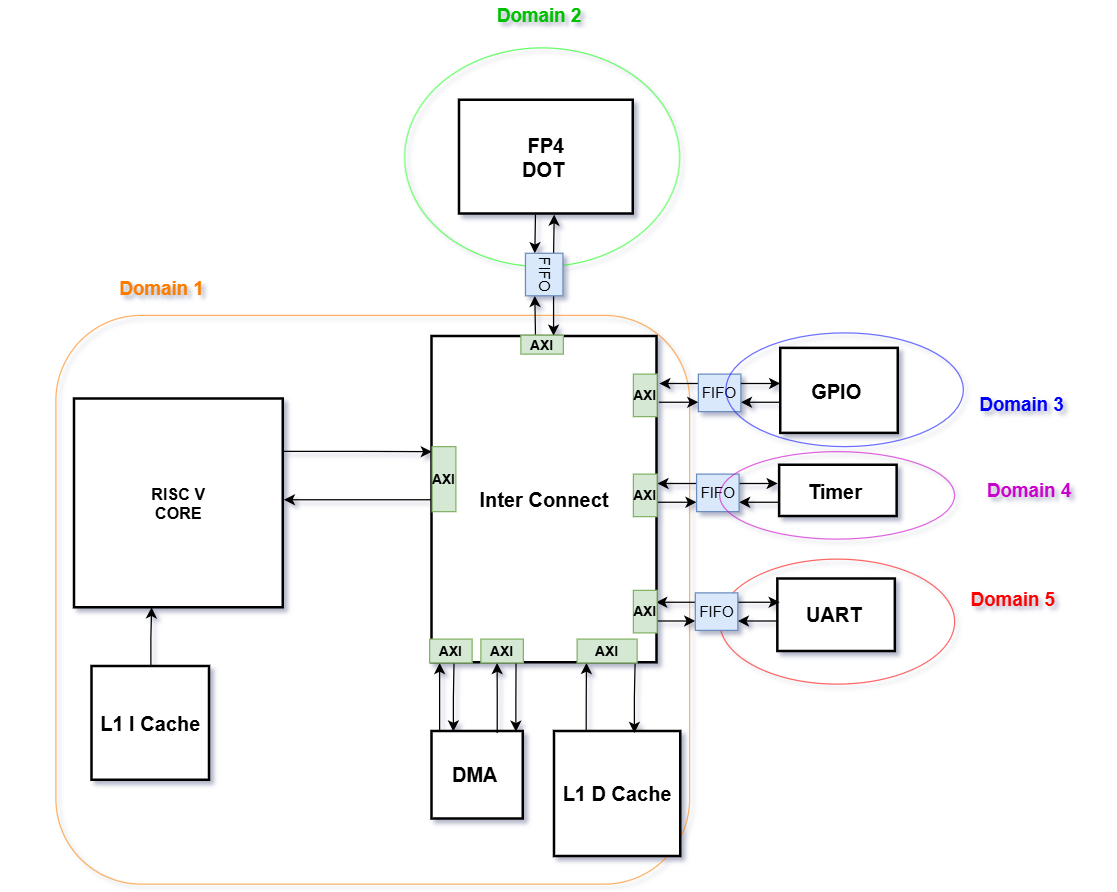
\includegraphics[width=0.92\linewidth]{benchmark.png}
\captionof{figure}{Nebula SoC benchmark: five asynchronous clock domains, each peripheral crossing into the AXI interconnect through a dedicated async FIFO.}
\end{center}

\begin{center}
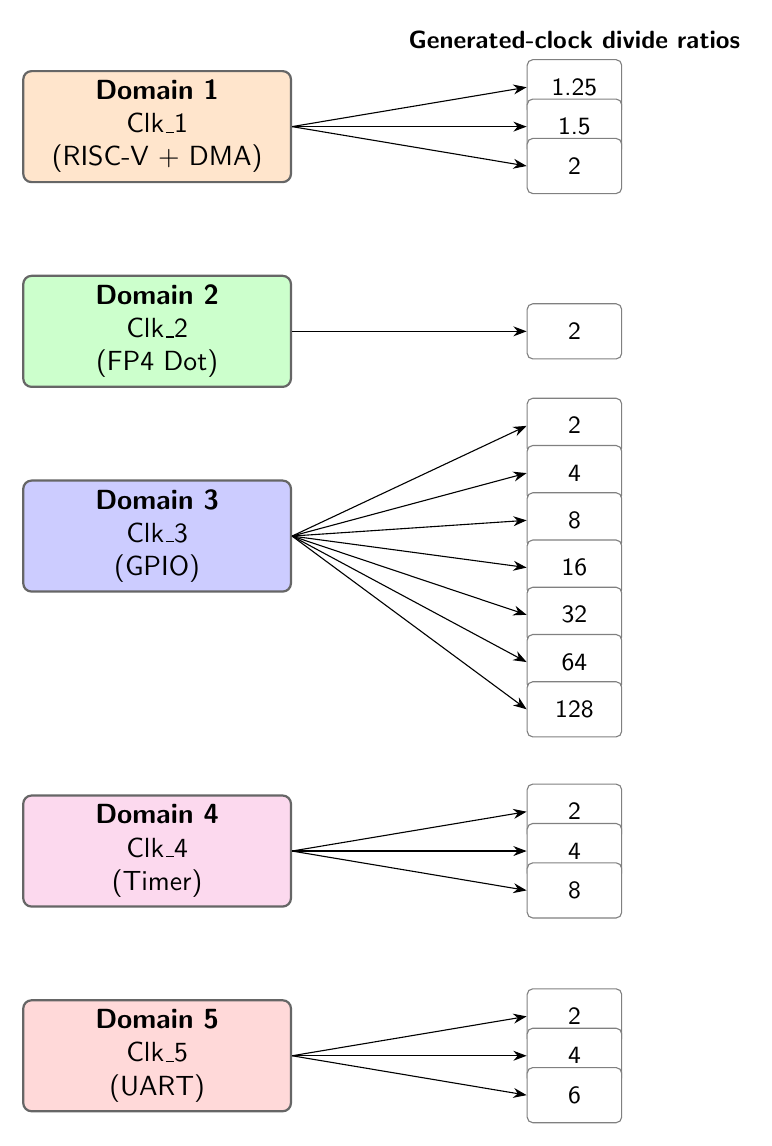
\includegraphics[width=0.55\linewidth]{clock_domains.png}
\captionof{figure}{Generated-clock divide ratios per domain --- 1.25/1.5/2 on domain 1, 2 on domain 2, seven octave steps (2 through 128) on domain 3, 2/4/8 on domain 4, 2/4/6 on domain 5.}
\end{center}

\section*{Implementation Plan: Files and Flow}

Every stage below is a concrete script against a concrete file, not an
abstract box --- matching the RTL$\rightarrow$Sign-off flow diagram this
abstract is built from.

\begin{enumerate}[leftmargin=1.4em, itemsep=4pt]

\item \textbf{RTL source.} Hand-written Verilog under
\texttt{rtl/} --- one file per block (\texttt{riscv\_core.v},
\texttt{fp4\_dot.v}, \texttt{gpio.v}, \texttt{timer.v}, \texttt{uart.v},
\texttt{axi\_interconnect.v}, \texttt{async\_fifo.v}, and one clock-divider
module per domain, including the fractional-ratio divider for domain~1)
plus one top-level \texttt{nebula\_soc.v} that instantiates and wires them.
A companion \texttt{nebula\_soc.sdc} defines all five \texttt{create\_clock}
masters, a \texttt{create\_generated\_clock} per divider ratio, and
\texttt{set\_clock\_groups -asynchronous} across every domain pair to mark
the CDC boundaries for STA.

\item \textbf{Lint.} \texttt{run\_lint.py} runs Verilator/slang against the
\texttt{.v} sources and fails the loop early on structural issues (unused
signals, width mismatches, latch inference) before spending synthesis time
on broken RTL. Output: a lint log; pass/fail gates progression to synthesis.

\item \textbf{Synthesis.} \texttt{run\_synth.py} wraps \texttt{run\_synth.tcl}
(Yosys), taking the RTL, the SDC, the sky130hd Liberty (\texttt{.lib}) and
LEF as input, and emitting a synthesized gate-level netlist
(\texttt{*\_synth.v}) plus an area/cell-count report.

\item \textbf{Timing/Area/Power gate.} \texttt{run\_sta.py} wraps
\texttt{run\_sta.tcl} (OpenSTA) against the synthesized netlist and SDC,
producing a structured JSON report (\path{artifacts/<run-id>_sta_report.json})
of ranked critical paths with slack --- this JSON is the literal input the
LLM reads, not a human-readable \texttt{.rpt}. If every path meets timing,
area, and power targets, the netlist proceeds to the equivalence gate;
otherwise the worst path's JSON entry and its RTL slice go to the LLM.

\item \textbf{GenAI RTL-fix loop.} \texttt{llm\_loop.py} calls the Claude API
with the critical-path JSON plus the relevant RTL module, constrained by tool-use
schema to return edited Verilog implementing exactly one of pipelining,
logic restructuring, retiming, or FSM re-encoding. The edit is written to
\path{artifacts/<run-id>/edit_<n>.v} and becomes the candidate RTL for the
next iteration --- never applied silently to the gold source.

\item \textbf{Equivalence check.} \texttt{run\_eqy.py} generates a
\texttt{.sby} config and runs EQY/SymbiYosys comparing the previous accepted
RTL against the new candidate. A mismatch discards the edit and returns
control to the LLM with an error report; a match promotes the candidate to
the new reference RTL and re-enters the synthesis/STA gate to confirm the
fix actually improved timing before it is allowed to proceed further.

\item \textbf{Floorplan through sign-off.} Once RTL is timing-clean and
equivalence-proven, OpenROAD-flow-scripts takes the netlist plus LEF/DEF/tech
files through floorplanning, global and detailed placement, clock tree
synthesis, global and detailed routing, and final STA, on the sky130hd PDK.
Each stage emits its own DEF and a timing/area/power report tagged with the
run ID; the advisory GenAI pass reads across all of them and emits a
suggestions document (\path{artifacts/<run-id>/suggestions.md}) without
touching RTL. Final output: GDSII, a matched before/after PPA report, and
the full equivalence-check trail, at sign-off.

\end{enumerate}

\section*{Evaluation Plan}

Nothing above has been run yet --- this is an abstract, not a results report.
What we commit to measuring once the loop runs on the benchmark:

\begin{itemize}[leftmargin=1.4em, itemsep=2pt]
\item \textbf{Closure rate:} how many of the injected critical paths close
inside a fixed iteration budget, out of the total injected.
\item \textbf{Slack recovered:} on paths that do close, how much slack comes
back, reported per-path, not averaged away.
\item \textbf{Failures reported too:} paths that don't converge in budget are
counted and shown, not omitted.
\item \textbf{Benchmark to beat:} ViTAD's~\cite{vitad} 73.68\% repair rate
against a 54.38\% plain-LLM baseline is the published number we'll compare
our actual results against once we have them --- not a target we're claiming
to have already hit.
\end{itemize}

\renewcommand{\refname}{References}
\noindent\textit{This project's architecture, benchmark design, and
evaluation plan were shaped by the following prior work.}

{\small
\begin{thebibliography}{99}

\bibitem{aieda} \emph{AiEDA: An Open-Source AI-Native EDA Framework}, 2024.
\url{https://arxiv.org/html/2412.09745v1}

\bibitem{autochip} S.~Thakur et al., \emph{AutoChip: Automating HDL Generation
Using LLM Feedback}, 2024. \url{https://arxiv.org/abs/2411.11856} ---
reference implementation: \url{https://github.com/shailja-thakur/AutoChip}

\bibitem{rethinking} \emph{Rethinking LLM-Based RTL Code Optimization Via
Timing Awareness}, 2025. \url{https://arxiv.org/abs/2507.16808}

\bibitem{symrtlo} \emph{SymRTLO: Enhancing RTL Code Optimization with LLMs and
Neuron-Inspired Symbolic Reasoning}, 2025.
\url{https://arxiv.org/abs/2504.10369}

\bibitem{vitad} \emph{ViTAD: Timing-Violation-Aware RTL Repair with LLMs},
2025. \url{https://arxiv.org/pdf/2508.13257}

\bibitem{timingllm} \emph{TIMINGLLM: RAG-Based FPGA Timing Closure with Large
Language Models.}

\bibitem{chipseek} \emph{ChipSeek: RL-Guided RTL Timing Closure}, 2025.
\url{https://arxiv.org/html/2507.04736v2}

\bibitem{assertions} \emph{Closing the Loop on LLM-Generated RTL Assertions},
2026. \url{https://arxiv.org/pdf/2606.21451}

\bibitem{gpextract} \emph{Timing-Driven Global Placement by Efficient Critical
Path Extraction}, 2025. \url{https://arxiv.org/abs/2503.11674}

\bibitem{regplace} \emph{A Machine Learning Framework for Register Placement
Optimization}, 2018. \url{https://arxiv.org/pdf/1801.02620}

\bibitem{edasurvey} \emph{Deep Representation Learning for Electronic Design
Automation: A Survey}, 2025. \url{https://arxiv.org/pdf/2505.02105}

\bibitem{sweagent} J.~Yang et al., \emph{SWE-agent: Agent-Computer Interfaces
Enable Automated Software Engineering.}
\url{https://github.com/SWE-agent/SWE-agent}

\bibitem{qoragent} \emph{Automated QoR Improvement in OpenROAD with Coding
Agents}, 2026. \url{https://arxiv.org/abs/2601.06268}

\bibitem{asicagent} A.~Allam, Y.~Mansour, M.~Shalan, \emph{ASIC-Agent: A
Multi-Agent System for Autonomous ASIC Design}, 2025.
\url{https://arxiv.org/abs/2508.15940}

\end{thebibliography}
}

\end{document}
